\chapter{Prototipo Funcional}

En este capítulo se describe el último prototipo del proyecto, el prototipo funcional. En él se expone todo lo referente a la implementación del servidor Erlang sobre la placa R-Pi, esto incluye: la creación del servidor base, la implementación de un servicio API REST, la creación de la interfaz del servidor y la implementación de la funcionalidad de lanzar la lectura de los sensores. Por último, se realizan pruebas de carga sobre el servidor para poner a prueba su rendimiento.

\section{Elección del servidor Web}

Existen múltiples opciones para crear servidores web usando Erlang, a continuación se describen algunos de los más comúnmente usados:
\begin{enumerate}
    \item \textbf{Yaws}: Es uno de los servidores web más populares en el entorno de Erlang y se destaca por su eficiencia y escalabilidad.
    \item \textbf{Cowboy}: Servidor web escrito en Erlang que ofrece un enfoque ligero y eficiente para el manejo de solicitudes HTTP. Es conocido por su rendimiento y flexibilidad, y se utiliza ampliamente en el desarrollo de aplicaciones web en Erlang.
    \item \textbf{MongooseIM}: Servidor de mensajería instantánea y chat en tiempo real. Está basado en el protocolo XMPP (Extensible Messaging and Presence Protocol) y ofrece capacidades de mensajería escalables y confiables.
    \item \textbf{RabbitMQ}: Servidor de mensajes y cola de tareas. Proporciona un sistema de mensajería robusto y escalable para el intercambio de datos entre diferentes componentes de una aplicación.
\end{enumerate}

A su vez existen bibliotecas y herramientas incluidas en el propio lenguaje como puede ser \textit{inets}, que proporciona una amplia gama de funcionalidades relacionadas con la infraestructura web y facilita el desarrollo de aplicaciones HTTP y otros protocolos web.

Debido a la naturaleza de este proyecto se ha decidido utilizar \textbf{Cowboy} ya que se trata de un servidor sencillo de usar y eficiente para este tipo de tareas, además es un servidor que soporta varios protocolos web como HTTP y WebSoquets y proporciona un sistema de enrutamiento flexible que permite asociar patrones de URL con funciones específicas, lo que será utilizado posteriormente para la funcionalidad de API REST . Para comenzar, se han seguido los pasos de instalación y creación de este tipo de servidores que nos ofrece la página oficial en su apartado <<Getting started>>, mediante estos podremos crear la base desde donde avanzar hacia el objetivo final de nuestro servidor funcional.

Un servidor Cowboy funciona siguiendo un modelo de concurrencia basado en actores y utiliza el sistema de concurrencia ligera de Erlang para manejar conexiones concurrentes de manera eficiente. A continuación, se explica de manera general como funciona:

\begin{enumerate}
    \item \textbf{Configuración}: En primer lugar, se realiza la configuración de Cowboy. Esto implica definir los puertos en los que el servidor escuchará las solicitudes entrantes, configurar enrutamiento y asociar funciones o módulos a rutas específicas.
    \item \textbf{Recepción de solicitudes}: Una vez que el servidor está configurado y en ejecución, comienza a escuchar las solicitudes entrantes en los puertos especificados. Cuando se recibe una solicitud HTTP, Cowboy la captura y la enruta a la función o módulo correspondiente según las reglas de enrutamiento definidas.
    \item \textbf{Enrutamiento}: Como se comentó anteriormente, Cowboy utiliza un sistema de enrutamiento flexible que permite asociar patrones de URL con funciones o módulos específicos. Esto se puede hacer mediante el uso de patrones de coincidencia o mediante la configuración manual de las rutas. Al recibir una solicitud, Cowboy verifica la ruta solicitada y la redirige a la función o módulo apropiado para su procesamiento.
    \item \textbf{Procesamiento de la solicitud}: Una vez que Cowboy ha determinado la función o módulo encargado de procesar la solicitud, pasa los datos de la solicitud (como los encabezados, el cuerpo y los parámetros) a dicha función o módulo. Aquí es donde se realiza la lógica de la aplicación para procesar la solicitud y generar una respuesta, en nuestro caso ejecutar un sensor, devolver datos o mostrar descripciones.
    \item \textbf{Generación de la respuesta}: La función o módulo encargado de procesar la solicitud en Cowboy genera una respuesta apropiada. Esto puede implicar la generación de contenido dinámico, la consulta de una base de datos o cualquier otra operación necesaria para construir la respuesta HTTP adecuada.
    \item \textbf{Envío de la respuesta}: Una vez generada la respuesta, Cowboy envía la respuesta HTTP al cliente que realizó la solicitud. Esto incluye enviar los encabezados HTTP adecuados y el cuerpo de la respuesta si corresponde.
\end{enumerate}

Este proceso se repite para cada solicitud entrante que recibe Cowboy. El servidor está diseñado para manejar múltiples solicitudes concurrentemente utilizando el modelo de concurrencia de Erlang y aprovechando la escalabilidad y eficiencia inherentes al lenguaje.

\cleardoublepage


\section{Creación del servidor Web}

\subsection{Objetivos de funcionalidad}

Tras el análisis de requisitos del proyecto se ha decidido crear un servidor que disponga de cierta funcionalidad y que esta sea fácilmente escalable, por ello se ha elegido el diseño de una API REST que, mediante la utilización de Cowboy, implementará un servidor que permita hacer lo siguiente:

\begin{enumerate}
    \item Acceso a una página de Inicio.
    \item Ver qué sensores se encuentran disponibles.
    \item Acceder a la descripción de cada uno de los sensores junto con su manual de uso.
    \item Lanzar la lectura de los sensores con valores por defecto.
    \item Lanzar la lectura de los sensores con la posibilidad de modificar sus argumentos de tiempo de lectura y ratio de lectura.
    \item Acceder a los archivos que almacenan los datos recibidos por los sensores.
\end{enumerate}

Los documentos que devolverá el servidor ya sean manuales o descripciones serán almacenadas en formato JSON. Los documentos que almacenan los datos de los sensores permanecerán en .txt.


\subsection{Configuración inicial}%
\label{sec:ConfigCowboy}

La configuración inicial del servidor Erlang implementado con Cowboy se realiza siguiendo los pasos de la sección <<Getting Started>> de la página ninenines.eu referenciada en \cite{Nines2012}. A continuación, se describirán los pasos seguidos para conseguir una pequeña aplicación de servidor que se utilizará como base desde la que avanzar hacia el objetivo final.

En primer lugar, debe crearse el directorio en el que almacenaremos nuestro servidor, para ello ejecutamos los siguientes comandos en el terminal de la placa R-Pi sobre el directorio en el que deseamos trabajar para crear el nuevo directorio y acceder a él.\\ 

\begin{lstlisting}[style=terminal]
$ mkdir hello_erlang
$ cd hello_erlang
\end{lstlisting}

El siguiente paso es realizar la descarga de Erlang.mk, esta herramienta proporcionará una forma simple de compilar, probar y gestionar dependencias para aplicaciones Erlang utilizando un enfoque basado en Makefile para definir el proceso de construcción y automatización de tareas comunes. Para descargar esta herramienta utilizaremos el comando\\

\begin{lstlisting}[style=terminal]
$ wget https://erlang.mk/erlang.mk
\end{lstlisting}

Tras realizar la descarga, se utiliza bootstrap para crear el entorno de la aplicación y su versión ejecutable con el comando siguiente.

\begin{lstlisting}[style=terminal]
make -f erlang.mk bootstrap bootstrap-rel
\end{lstlisting}

Una vez realizados estos pasos podemos construir y lanzar el servidor pero aún faltarán pasos para que este funcione correctamente.\\

La configuración de Cowboy comienza por modificar el Makefile para que el sistema detecte que vamos a usar los plugins y dependencias de Cowboy junto con su respectiva versión. El Makefile debe quedar de la siguiente manera:\\

\lstset{language=C, breaklines=true, basicstyle=\sffamily\footnotesize}
\begin{lstlisting}[frame=single]
PROJECT = hello_erlang

DEPS = cowboy
dep_cowboy_commit = 2.6.3

DEP_PLUGINS = cowboy
include erlang.mk
\end{lstlisting}

El siguiente paso es definir las rutas que Cowboy utilizará para enlazar con los módulos del servidor que realizarán las acciones, también llamados <<handlers>>, para ello se modifica el archivo hello\_erlang\_app.erl que se ha creado automáticamente en el directorio /src. En esta primera parte de la configuración únicamente le introduciremos la ruta raíz <</>> que se redirigirá a hello\_handler.erl, además se añade la configuración que lanzará el servidor en localhost sobre el puerto 8080, todo ello en la función start/2. El código de hello\_erlang\_app.erl quedaría como sigue:\\

\lstset{language=Erlang, breaklines=true, basicstyle=\sffamily\footnotesize}
\begin{lstlisting}[frame=single]
start(_Type, _Args) ->
    Dispatch = cowboy_router:compile([
        {'_', [{"/", hello_handler, []}]}
    ]),
    {ok, _} = cowboy:start_clear(my_http_listener,
        [{port, 8080}],
        #{env => #{dispatch => Dispatch}}
    ),
    hello_erlang_sup:start_link().
\end{lstlisting}

Por último, debe crearse el handler hello\_handler.erl que será quien responda a la llamada <</>> desde el servidor. Para esta configuración inicial únicamente debemos esperar una respuesta correcta por parte del servidor y que este devuelva <<Hello Erlang!>>. Para ello, se introducirá la siguiente función en hello\_handler.erl.\\

\lstset{language=Erlang, breaklines=true, basicstyle=\sffamily\footnotesize}
\begin{lstlisting}[frame=single]
init(Req0, State) ->
    Req = cowboy_req:reply(200,
        #{<<"content-type">> => <<"text/plain">>},
        <<"Hello Erlang!">>,
        Req0),
    {ok, Req, State}.
\end{lstlisting}

Tras estos pasos ya tenemos disponible el funcionamiento más básico del servidor Erlang utilizando Cowboy, a partir de aquí podremos ir añadiendo funcionalidad para que cumpla los requisitos del proyecto. En los siguientes apartados de esta sección se describirán los puntos principales del proceso de creación del mismo.

\subsection{Diseño de la API REST}

El esquema de la API REST será sencillo y se basará en carpetas como los sistemas operativos habituales. A continuación se describirá el diseño de la API utilizando un árbol de directorios.\\

\dirtree{%
.1 /.
.2 sensores.
.3 magnetómetro.
.4 launch.
.4 data.
.5 angulos.txt.
.3 ultrasonido.
.4 launch.
.4 data.
.5 distancias.txt.
}

A través de este esquema se puede observar el funcionamiento del servidor. En primer lugar, al acceder al él nos encontramos en la carpeta raíz, que nos mostrará una introducción al servidor y ofrecerá el acceso a la descripción de los sensores. En caso de acceder a la carpeta /sensores nos encontraremos con la descripción de las posibilidades de manejo del servidor sobre los diferentes sensores disponibles.

Tras elegir alguno de los sensores accediendo mediante su nombre (ej: /sensores/ultrasonido) dispondremos de una descripción detallada del mismo junto con un manual que describirá cómo ejecutar su lectura, ya sea de manera predeterminada o personalizada así como la forma de acceder a los datos obtenidos. Por último, el directorio <<../data>> nos permitirá visualizar al archivo txt que contendrá los últimos datos leídos por el sensor seleccionado.


\subsection{Descripción de sensores}

La descripción de los sensores y el manual de uso de la API REST se creará en lenguaje JSON, posteriormente, estos archivos serán referenciados desde el servidor para que sea el navegador quien los analice y los muestre en este formato.

Se han creado tres archivos JSON, uno para cada sensor utilizado y otro para la página que muestra las posibilidades de ejecución de los mismos. A continuación se muestra un ejemplo del archivo que se visuaizará en caso de acceder al directorio <</sensores>>, este ofrece un diagrama sobre las diferentes posibilidades de acceso desde este directorio.
\clearpage
\lstset{language=JSON, breaklines=true, basicstyle=\footnotesize}
\begin{lstlisting}[frame=single, caption=sensores.json]
{
  "sensores": [
    {
      "name": "Sensor Magnetometro HMC5983",
      "specs": "http://localhost:8080/sensores/magnetometro",
      "default_launch": "http://localhost:8080/sensores/magnetometro/launch",
      "custom_launch" : "http://localhost:8080/sensores/magnetometro/launch?time=X&frec=Y",
      "last_data" : "http://localhost:8080/sensores/magnetometro/data"
    },
    {
      "name": "Sensor de Distancia HJC-SR04",
      "specs": "http://localhost:8080/sensores/ultrasonido",
      "default_launch": "http://localhost:8080/sensores/ultrasonido/launch",
      "custom_launch" : "http://localhost:8080/sensores/ultrasonido/launch?time=X&frec=Y",
      "last_data" : "http://localhost:8080/sensores/ultrasonido/data"
    }
  ]
}
\end{lstlisting}


\subsection{Ejecución de sensores}

Los sensores deben poder ejecutarse desde el servidor, por ello se ha creado un módulo que se ocupa únicamente de realizar estas ejecuciones, se trata de launch\_handler.erl. En esta sección se describirá el código de este módulo.

En primer lugar, ha de tenerse en cuenta como se ejecutan los sensores para posteriormente tratar de realizar esta ejecución desde el servidor. Los sensores utilizan un código escrito en lenguaje C, descrito en el Capítulo~\ref{cap.prototipoExploracion}, este código necesita dos argumentos para ejecutarse y almacena los datos en un archivo .txt. 

El lugar de almacenamiento del código es la placa de desarrollo, al igual que los sensores que están conectados a la misma, por esto la tarea del servidor es ejecutar este código en la placa R-Pi pasándole los argumentos necesarios para que, al finalizar la ejecución, el servidor pueda acceder al archivo creado con los datos leídos por el sensor. A continuación se explicará detalladamente el funcionamiento del módulo Erlang creado para las tareas mencionadas. A este módulo se accederá al lanzar <<../launch>> desde el servidor eligiendo con anterioridad el tipo de sensor a lanzar.

En primer lugar, se realiza la exportación de las funciones a utilizar, se trata de  \textit{init/2}, \textit{execute\_ultrasonido/2}, \textit{execute\_magnetometro/2}, \textit{allowed\_methods/2} y \textit{content/2}. Estas funciones se encuentran descritas a continuación:

\begin{itemize}
    \item \textbf{init/2}: Encargada de inicializar la respuesta a una solicitud HTTP con un código de estado 200 y establecer el tipo de contenido como <<text/plain>>.
    \item \textbf{allowed\_methods/2}: Especifica los métodos HTTP permitidos para una solicitud determinada, en este caso GET, POST y DELETE.
    \item \textbf{content/2}: Se utiliza para procesar las solicitudes HTTP entrantes y determinar cómo responder. Dependiendo de la ruta y los parámetros de la consulta, se ejecutan las funciones correspondientes para lanzar la ejecución de los programas externos y recopilar datos de los sensores. En caso de no recibir parámetros se establecen por defecto, de esta manera cuando llega únicamente una petición de lanzamiento de un sensor sin especificar parámetros de lanzamiento, no ocurre un error sino que se llama a la función de ejecución del sensor con estos parámetros por defecto.
    \item \textbf{execute\_ultrasonido/2} : Responsable de la ejecución de los comandos externos mediante el uso de ports Erlang, esta función es llamada a través de \textit{content/2} cuando se recibe la solicitud\\ <</ultrasonido/launch>> y necesita los parámetros Time y Frec para realizar la ejecución del código que lanza la lectura del sensor. Por último, también llama a \textit{receive\_data}, que recibirá la respuesta del código ejecutado.

    \item \textbf{execute\_magnetometro/2} : Funciona de manera similar a \textit{execute\_ultrasonido/2} solo que esta ejecuta el código del sensor magnetómetro y es llamada cuando se recibe la solicitud\\ <</magnetometro/launch>>.
    
    \item \textbf{receive\_data/1}: Se encarga de recibir los datos enviados por los programas externos a través del port Erlang y realizar acciones específicas según los datos recibidos. Por ejemplo, muestra mensajes de éxito cuando los datos se han recopilado correctamente. Para saber que todo ha ido bien utiliza la última salida de los programas C como indicador de fin de ejecución.
\end{itemize}

   El uso de un port Erlang permite la comunicación y la interoperabilidad con programas escritos en otros lenguajes de programación, como es el caso de C. El uso de port es sencillo y consta de varios pasos:
   \begin{enumerate}
       \item Definir el comando o programa externo a ejecutar y determinar su ruta así como sus posibles argumentos.
       \item Abrir el port utilizando la función <<open\_port/2>>, esta función toma como argumento una tupla que especifica como se debe lanzar el programa externo, incluyendo el comando a ejecutar y cualquier opción adicional.
       \item Procesar los datos recibidos: Se utiliza la función \textit{receive} para recibir y procesar los datos enviados por el programa externo a través del port.
   \end{enumerate}

\lstset{language=Erlang, breaklines=true, basicstyle=\sffamily\footnotesize}
\begin{lstlisting}[frame=single, caption=launch\_handler.erl]
-module(launch_handler).

-export([
    init/2,
    execute_ultrasonido/2,
    execute_magnetometro/2,
    allowed_methods/2,
    content/2
]).

init(Req0, State) ->
    Req = cowboy_req:reply(200,
        #{<<"content-type">> => <<"text/plain">>},
        content(cowboy_req:path(Req0), cowboy_req:qs(Req0)),
        Req0),
    {ok, Req, State}.

allowed_methods(Req, State) ->
    Methods = [<<"GET">>, <<"POST">>, <<"DELETE">>],
    {Methods, Req, State}.
    
execute_ultrasonido(Time, Frec) ->
    Command = "/home/martorn/Desktop/distanceSensor/ultrasonido " ++ Time ++ " " ++ Frec,
    Port = open_port({spawn, Command}, [stream]),
    receive_data(Port).

execute_magnetometro(Time, Frec) ->
    Command = "sudo /home/martorn/Desktop/hmc5983_i2c/CabeceoArchivo/cabeceoArchivo " ++ Time ++ " " ++ Frec,
    Port = open_port({spawn, Command}, [stream]),
    receive_data(Port).

receive_data(Port) ->
    receive
        {Port, {data, Data}} when Data == "UltOK" -> % Utiliza "UltOK" como indicador de fin de ejecucion.
          "Recogida de datos finalizada correctamente!, accede al archivo a traves de http://localhost:8080/sensores/ultrasonido/data";
        
        {Port, {data, Data}} when Data == "MagOK" -> % Utiliza "MagOK" como indicador de fin de ejecucion.
        "Recogida de datos finalizada correctamente!, accede al archivo a traves de http://localhost:8080/sensores/magnetometro/data";
        
        {Port, {data, Data}} ->
		io:format("~p~n", [Data]),
            receive_data(Port);
        {Port, {error, Reason}} ->
		Reason,
            io:format("Error al recibir datos del programa C: ~p~n", [Reason])
        end.
    
content(Path, QueryString) when Path == <<"/sensores/ultrasonido/launch">> ->
	
	Params = cow_qs:parse_qs(QueryString), %Divide la parte del query en cada uno de sus argumentos
	io:format("Params: ~p~n", [Params]),
	TimeBin = proplists:get_value(<<"time">>, Params, <<"5">>), %Obtiene el valor de time en binario, formato <<"x">>
	FrecBin = proplists:get_value(<<"frec">>, Params, <<"0.5">>), %Obtiene el valor de frec en binario, formato <<"x">>
	Time = binary_to_list(TimeBin), %Pasa el argumento a list para que la funcion que ejecuta el codido pueda leerlo
	Frec = binary_to_list(FrecBin),
	io:format("Time: ~p~n", [Time]),
	io:format("Frec: ~p~n", [Frec]),
    execute_ultrasonido(Time, Frec); %Se lanza la funcion con los argumentos especificados
		
	
content(Path, QueryString) when Path == <<"/sensores/magnetometro/launch">> ->
	
	Params = cow_qs:parse_qs(QueryString), %Divide la parte del query en cada uno de sus argumentos
	io:format("Params: ~p~n", [Params]),
	TimeBin = proplists:get_value(<<"time">>, Params, <<"5">>), %Obtiene el valor de time en binario, formato <<"x">>
	FrecBin = proplists:get_value(<<"frec">>, Params, <<"0.5">>), %Obtiene el valor de frec en binario, formato <<"x">>
	Time = binary_to_list(TimeBin), %Pasa el argumento a tipo list para que la funcion que ejecuta el codido pueda leerlo
	Frec = binary_to_list(FrecBin),
	io:format("Time: ~p~n", [Time]),
	io:format("Frec: ~p~n", [Frec]),
    execute_magnetometro(Time, Frec); %Se lanza la funcion con los argumentos especificados
  
content(_, _) ->
    <<"Not Found">>.
\end{lstlisting}

\subsection{Muestra de datos}

La visualización de los datos leídos por cada uno de los sensores la realiza el módulo data\_handler.erl que es llamado desde hello\_erlang\_app.erl cuando se realiza la solicitud HTTP con la dirección\\ <</sensores/SensorX/data>>. Su código es sencillo, cuando llega una solicitud a este módulo determina de qué sensor se trata y realiza la lectura del archivo creado por este sensor, el cual se almacena en una ubicación específica de la placa R-Pi. \\

\lstset{language=Erlang, breaklines=true, basicstyle=\sffamily\footnotesize}
\begin{lstlisting}[frame=single, caption=data\_handler.erl]

-module(data_handler).

-export([
    init/2,
    allowed_methods/2,
    content/2
]).

init(Req0, State) ->
    Req = cowboy_req:reply(200,
        #{<<"content-type">> => <<"text/plain">>},
        content(cowboy_req:path(Req0), cowboy_req:qs(Req0)),
        Req0),
    {ok, Req, State}.

allowed_methods(Req, State) ->
    Methods = [<<"GET">>, <<"POST">>, <<"DELETE">>],
    {Methods, Req, State}.
    
content(Path, _) when Path == <<"/sensores/ultrasonido/data">> -> 
     {ok, Data} = file:read_file("/home/martorn/Desktop/hello_erlang/src/sensorData/distancias.txt"),
        Data;
        
content(Path, _) when Path == <<"/sensores/magnetometro/data">> ->
     {ok, Data} = file:read_file("/home/martorn/Desktop/hello_erlang/src/sensorData/angulosCabeceo.txt"),
        Data;

content(_, _) ->
    <<"Not Found">>.
\end{lstlisting}
\subsection{Servidor final}

El servidor final consta de siete módulos que realizan las funcionalidades deseadas, en esta sección se describirá cada uno de ellos y se mostrará el código de aquellos no mostrados anteriormente y que se consideran importantes:

\begin{enumerate}
    \item \textbf{hello\_erlang\_sup.erl}: Responsable de administrar los procesos y la tolerancia a fallos de la aplicación. Se utiliza la estrategia <<one\_for\_one>> para reiniciar los procesos en caso de fallos.
    \item \textbf{hello\_erlang\_app.erl}: Contiene la información de enrutamiento del servidor, es el módulo encargado de redirigir a cada uno de los controles dependiendo de la ruta solicitada. Es aquí donde debemos cambiar la ip y el puerto en el que se lanzará el servidor en caso de ser necesario.
    \item \textbf{hello\_handler.erl}:  Página de inicio del servidor, se almacena en el directorio raíz. Muestra una bienvenida y las posibilidades de acceso (/sensores).
    \item \textbf{not\_found\_handler.erl}: Módulo encargado de mandar un mensaje de <<No encontrado>> en caso de que la URL solicitada no se encuentre disponible en el servidor.
    \item \textbf{update\_handler.erl}: Controlador responsable de mostrar las descripciones y manuales de los sensores almacenados en JSON.
     \item \textbf{data\_handler.erl}: Da acceso a los diferentes archivos de datos leídos por los sensores.
      \item \textbf{launch\_handler.erl}: Controlador encargado de lanzar la ejecución de los diferentes sensores conectados a la placa R-Pi.
\end{enumerate}

\lstset{language=Erlang, breaklines=true, basicstyle=\sffamily\footnotesize}
\begin{lstlisting}[frame=single, caption=hello\_erlang\_sup.erl]
-module(hello_erlang_sup).
-behaviour(supervisor).

-export([start_link/0]).
-export([init/1]).

start_link() ->
	supervisor:start_link({local, ?MODULE}, ?MODULE, []).
 
init([]) ->
	Procs = [],
	{ok, {{one_for_one, 1, 5}, Procs}}.
\end{lstlisting}

\vspace{10mm}

\lstset{language=Erlang, breaklines=true, basicstyle=\sffamily\footnotesize}
\begin{lstlisting}[frame=single, caption=hello\_erlang\_app.erl]
-module(hello_erlang_app).
-behaviour(application).

-export([start/2]).
-export([stop/1]).

start(_Type, _Args) ->
    Dispatch = cowboy_router:compile([
        {'_', [
			{"/", hello_handler, []},
			{"/sensores", update_handler, []},
			{"/sensores/ultrasonido", update_handler, []},
			{"/sensores/ultrasonido/data", data_handler, []},
			{"/sensores/magnetometro", update_handler, []},
			{"/sensores/magnetometro/data", data_handler, []},
			{"/sensor", update_handler, []},
			{"/sensores/magnetometro/launch", launch_handler, []},
			{"/sensores/ultrasonido/launch", launch_handler, []},
			{'_', not_found_handler, []}  % Ruta por defecto (Not Found)
			]}
    ]),
    {ok, _} = cowboy:start_clear(my_http_listener,
        [{port, 8080},{ip, {192, 168, 1, 15}}],
        #{env => #{dispatch => Dispatch}}
    ),
    hello_erlang_sup:start_link().
    
stop(_State) ->
	ok.
\end{lstlisting}

\vspace{10mm}

\lstset{language=Erlang, breaklines=true, basicstyle=\sffamily\footnotesize}
\begin{lstlisting}[frame=single, caption=update\_handler.erl]
-module(update_handler).

-export([
    init/2,
    allowed_methods/2,
    content/2
]).

init(Req0, State) ->
    Req = cowboy_req:reply(200,
        #{<<"content-type">> => <<"application/json">>},
        content(cowboy_req:path(Req0), cowboy_req:qs(Req0)),
        Req0),
    {ok, Req, State}.

allowed_methods(Req, State) ->
    Methods = [<<"GET">>, <<"POST">>, <<"DELETE">>],
    {Methods, Req, State}.
    
    
content(Path, _) when Path == <<"/sensores">> ->
    {ok, Data} = file:read_file("/home/martorn/Desktop/hello_erlang/src/text/sensores.json"),
        Data;

content(Path, _) when Path == <<"/sensores/magnetometro">> ->
     {ok, Data} = file:read_file("/home/martorn/Desktop/hello_erlang/src/text/magnetometro.json"),
        Data;

content(Path, _) when Path == <<"/sensores/ultrasonido">> ->
    {ok, Data} = file:read_file("/home/martorn/Desktop/hello_erlang/src/text/ultrasonido.json"),
        Data;
                
content(_, _) ->
    <<"Not Found">>.
\end{lstlisting}

\section{Pruebas de carga sobre el servidor Web}
\subsection{Configuración de los escenarios}
La cantidad de usuarios simultáneos estimada sobre el servidor es muy baja ya que se trata de un sistema pequeño y pensado para un grupo limitado de usuarios, aún así se ha decidido poner a prueba el servidor Cowboy implementado sobre Raspberry-Pi para demostrar como funciona en casos de alta concurrencia y si es capaz de obtener un rendimiento adecuado. 

Para realizar estas pruebas de carga se ha utilizado la herramienta Apache Jmeter, descrita en la Sección~\ref{JMETER}. El primer paso es crear el escenario de la prueba, en este caso estudiaremos dos, uno con 100 usuarios (mucho más de lo habitual) y otro con 15000 (poniendo a prueba el servidor). En ambas pruebas los usuarios accederán todos a la vez (tiempo de subida = 1), además la prueba con 15000 hilos también se hará con un tiempo de subida de 10 segundos para ver como el servidor gestiona tantos usuarios sin acceder todos a la vez.

Para crear el escenario de prueba en la plataforma JMeter debe crearse un <<Thread Group>> dentro del que se crearán las muestras y se establecerán los <<listeners>> o escuchadores que nos ofrecerán los datos obtenidos en diferentes formatos. Nuestra muestra se basará en peticiones HTTP, por ello se añade como sampler <<HTTP Request>> y se configura para leer en el índice de nuestro servidor como se puede observar en la Figura~\ref{fig:JmeterConfig} 

\begin{figure}[h]
\centering
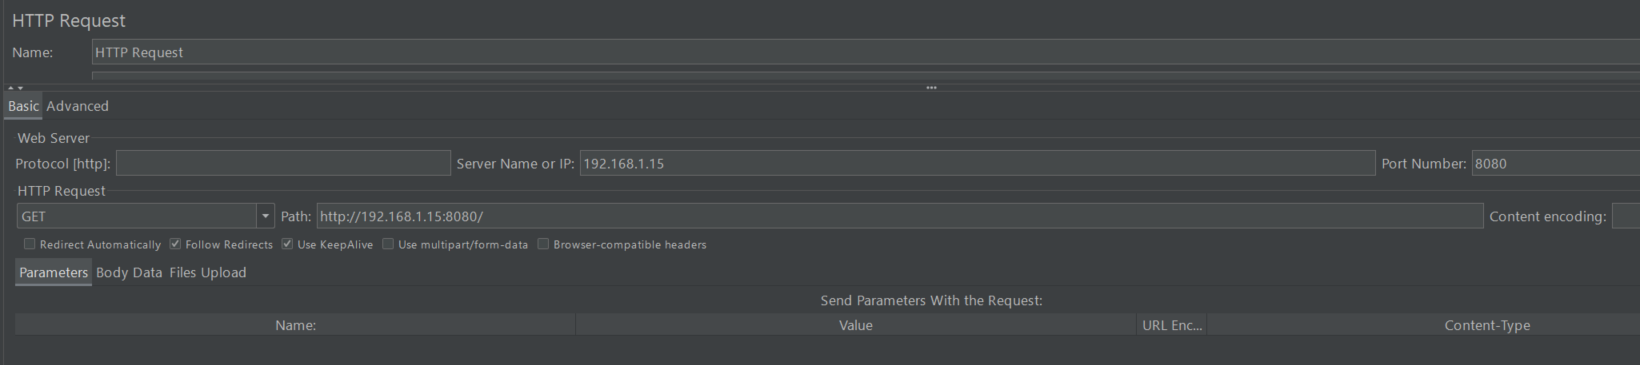
\includegraphics[scale=0.52]{images/configJmeter.png}
\caption[Configuración HTTP Request JMeter]{Configuración de las peticiones HTTP en Apache JMeter. Campos a tener en cuenta: Server name, Port Number, HTTP Request y Path.}%
\label{fig:JmeterConfig}
\end{figure}

En cuanto a la elección de los <<listeners>> se han seleccionado los siguientes debido a la utilidad de sus resultados:
\begin{itemize}
    \item View Results Tree: Nos ofrece cada una de las respuestas obtenidas de las peticiones HTTP, dentro de ellas podemos observar sus detalles.
    \item Agregate Report: Refleja una tabla con el resumen general del conjunto de las muestras obtenidas: Muestras, media, latencia, error, rendimiento... etc
    \item Response Time Graph: Devuelve un gráfico del tiempo de respuesta a lo largo del tiempo de muestreo
\end{itemize}
A mayores se ha instalado el pluging \textit{PerfMon} (Servers Performance Monitoring) que ofrece algunos gráficos más avanzados que pueden resultar interesantes, como los siguientes:

\begin{itemize}
    \item Active Threads Over Time: Gráfica que describe como los hilos han ido activándose a lo largo de la muestra. Proporciona una visión de como varía la carga de trabajo a lo largo del tiempo, lo que puede ayudar a identificar patrones de uso y momentos de mayor demanda en el sistema.
    \item Response Latencies Over Time: Esta gráfica analiza las latencias de respuesta obtenidas durante la ejecución de las pruebas. La latencia se refiere al tiempo transcurrido desde que se envía una solicitud hasta que se recibe la respuesta correspondiente. Este gráfico permite identificar los momentos en los que se producen retrasos en las respuestas del sistema y puede ayudar a detectar cuellos de botella o problemas de rendimiento.
    \item Bytes Throughput Over Time: Este gráfico muestra la cantidad de bytes transferidos en el sistema a lo largo del tiempo. Proporciona información sobre el rendimiento de la transferencia de datos en el sistema, lo que puede ser útil para evaluar la capacidad de la red o identificar problemas de ancho de banda.    
\end{itemize}

En la Figura~\ref{fig:listeners} se puede observar la lista de todos los listeners seleccionados.

\begin{figure}[h]
\centering
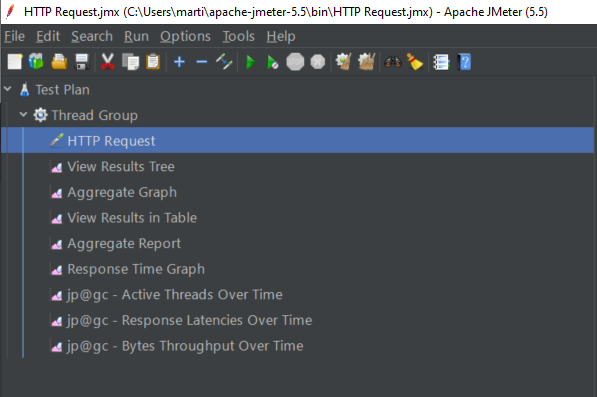
\includegraphics[scale=0.8]{images/listeners.png}
\caption[Listeners seleccionados]{Detalle de los tipos de clientes (\emph{Listeners}) utilizados en este escenario mediante Apache JMeter.}%
\label{fig:listeners}
\end{figure}

\subsection{Análisis de resultados}

A continuación, se mostrarán y analizaran los resultados obtenidos de las pruebas de carga realizadas sobre el servidor. Estos datos se mostrarán mediante las tablas y gráficas que ofrecen los propios listeners tras la finalización de las pruebas. 

\subsubsection{Escenario con 100 usuarios}


La Tabla~\ref{tab:100User} muestra los datos más interesantes del listener \textit{Agregate Report} obtenidos con la prueba que ha lanzado peticiones de 100 usuarios con un periodo de subida de 1 segundo (todos entran a la vez). Se trata de los tiempos de respuesta medidos en milisegundos por parte de la herramienta. Como puntos importantes de estos resultamos observamos que el error ha sido del 0\% y que las 100 peticiones se han resuelto en menos de 1 segundo, obteniendo así un rendimiento de 120 peticiones por segundo con un máximo de latencia de 90 milisegundos. En la Figura~\ref{fig:latencia100} puede observarse como este pico de latencia máximo aparece cuando al inicio de la prueba ya que es el momento en el que los 100 usuarios acceden al mismo tiempo, pero, a simple vista, puede verse que el servidor las resuelve de manera instantánea reduciendo la latencia a una media de 15 milisegundos hasta finalizar. 
En cuanto a la cantidad de Bytes recibidos y enviados, en la Figura~\ref{fig:respuestaJmeter} se puede observar cuál es la respuesta recibida por parte del servidor, se trata del texto plano que ofrece el servidor como bienvenida al acceder a su directorio raíz.\\

\begin{table}[h]
\begin{center}
\sffamily\small
\begin{tabular}{|c|c|c|c|c|c|c|c|}
\rowcolor{gray!20}
\hline
Muestras & Media & Mínimo & Máximo & \% Error & Rendimiento & KB/s Recibidos & KB/s enviados \\
\hline
100 & 26 & 6 & 90 & 0.00\% & 120.5/s & 42.71 & 14.35 \\
\hline
\end{tabular}
\caption[Salida <<Agregate Report>> con 100 hilos]{Datos obtenidos por el listener <<Agregate Report>> tras las pruebas realizadas con 100 usuarios y un tiempo de subida de 1 segundo, tiempos de respuesta en milisegundos}%
\label{tab:100User}
\end{center}
\end{table}


\begin{figure}[h]
\centering
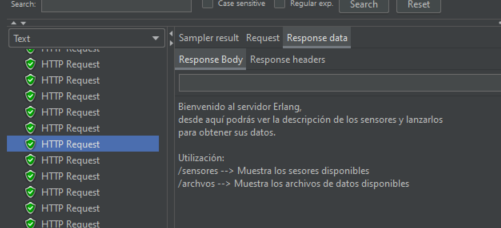
\includegraphics{images/respuestaJmeter.png}
\caption[Detalles de una HTTP Request obtenida]{Detalle de la respuesta obtenida por parte del servidor a todas las peticiones realizadas por la prueba de carga desde Apache JMeter.}%
\label{fig:respuestaJmeter}
\end{figure}


\begin{figure}[h]
\centering
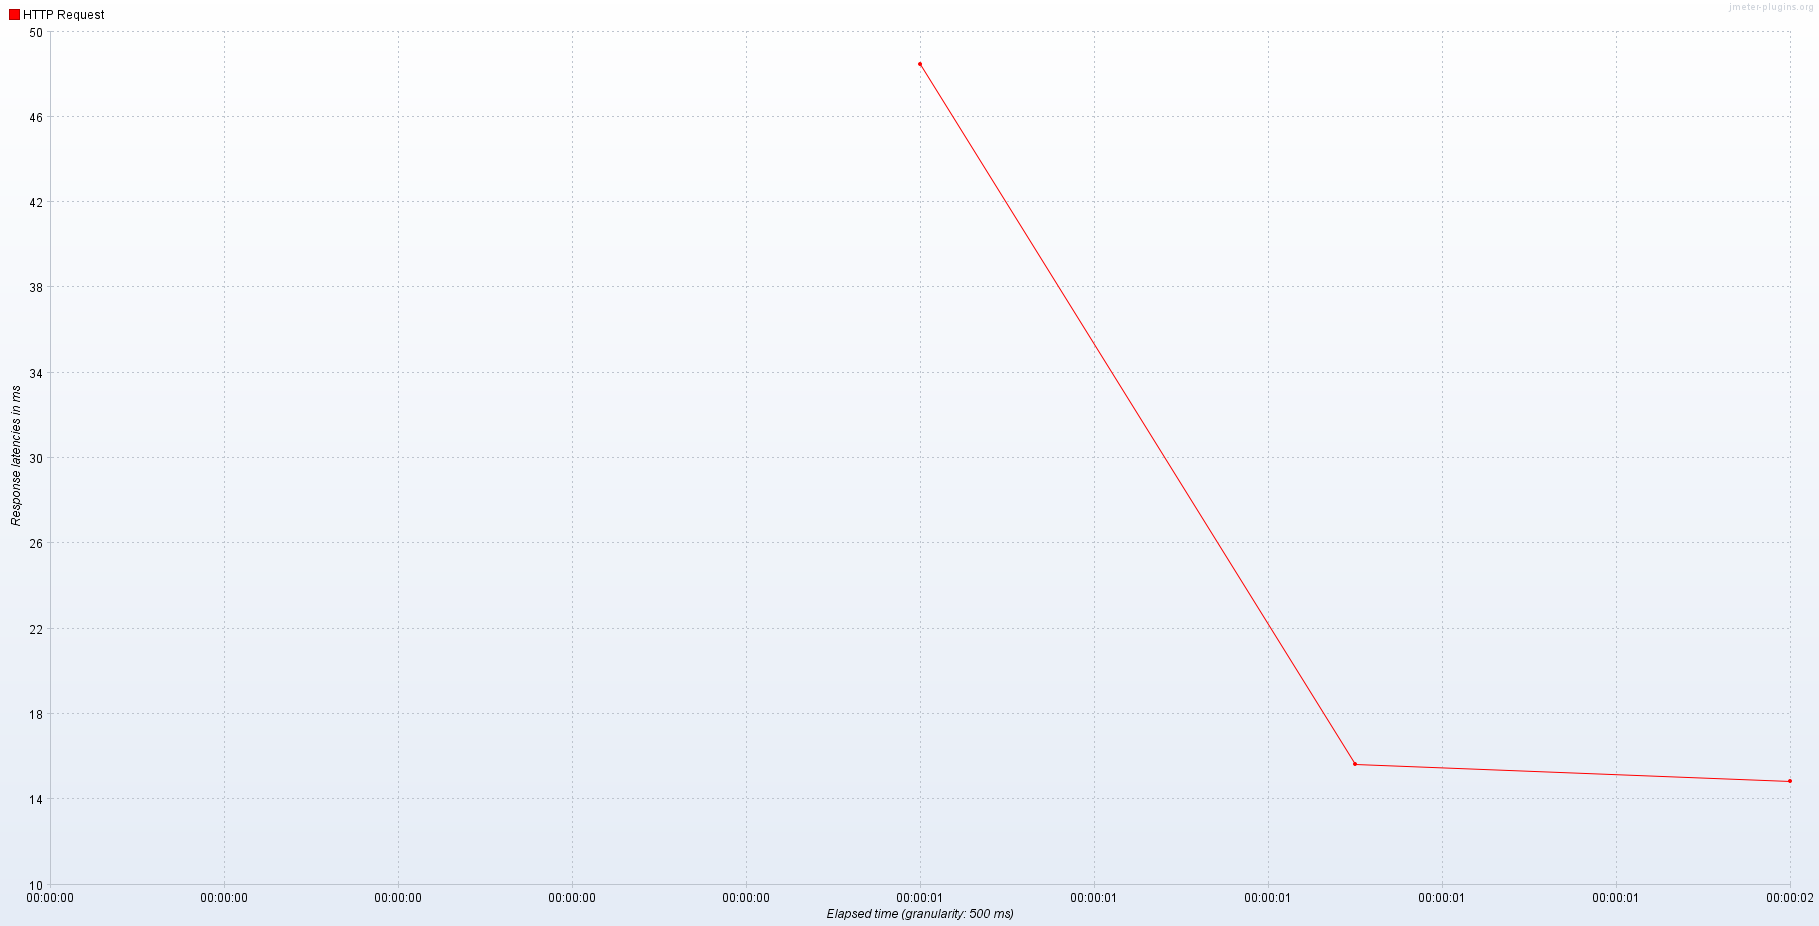
\includegraphics[scale=0.28]{images/latenciaGraf100.png}
\caption[Evolución de la latencia con 100 usuarios]{Evolución de la latencia en resolución de las peticiones desde 0 hasta 100 usuarios. Eje X medido en {\ttfamily hh:mm:ss} y eje Y medido en milisegundos.}%
\label{fig:latencia100}
\end{figure}



\subsubsection{Escenario con 15000 usuarios}

La Tabla~\ref{tab:15000User} muestra los datos más interesantes del listener \textit{Agregate Report} obtenidos con la prueba que ha lanzado peticiones de 15000 usuarios con un periodo de subida de 1 segundo (todos entran a la vez). Se trata de los tiempos de respuesta medidos en milisegundos por parte de la herramienta.

Como puntos importantes de estos resultamos observamos que se ha obtenido un error del 2,09\% por lo que en algún punto de la prueba se ha superado la cuota del servidor, para obtener más información sobre este fallo debe analizarse la salida obtenida por el terminal de ejecución el servidor representada en la Figura~\ref{fig:warning}, en ella aparece un Warning que se repite durante toda la prueba <<Ranch acceptor reducing accept rate: out of file descriptors>>, este aviso nos indica que el servidor ha llegado a su límite de descriptores, los descriptores de archivo son recursos limitados en un sistema operativo y se utilizan para representar archivos, sockets y otros objetos que pueden ser leídos o escritos. Cuando un servidor alcanza el límite de descriptores de archivo, no puede aceptar nuevas conexiones y, por lo tanto, reduce su tasa de aceptación, posteriormente veremos como solucionar esto en caso de necesitar tal capacidad de resolución de peticiones.

Por otro lado, el rendimiento del servidor ha sido muy alto, se han resuelto una media de 2318 peticiones por segundo lo cual indica una gran capacidad de resolución de peticiones simultáneas por parte de Cowboy. A continuación, analizaremos la gráfica obtenida de la evolución de la latencia a lo largo de la prueba.

En la Figura~\ref{fig:latencia15k} puede observarse como la latencia ha ido en aumento a lo largo del tiempo. Se ha dividido la gráfica en tres partes: 
\begin{itemize}
    \item \textbf{(1)}: En esta primera sección que abarca los dos primeros segundos de la prueba, la latencia ha ido subiendo progresivamente según han ido creándose los hilos.
    \item \textbf{(2)}: Del segundo 2 al 5 podemos ver un aumento más escalonado de la latencia, esto se debe a que se están resolviendo muchas de las peticiones entrantes pero al seguir entrando gran cantidad de ellas ocurren picos de latencia.
    \item \textbf{(3)}: A partir del segundo 6 el servidor se satura y el tiempo de respuesta aumenta de manera vertical hasta finalizar la prueba, provocando así ciertos errores. Es en este punto en el que aparecen los Warning comentados anteriormente indicando que la cuota de descriptores de archivo ha llegado a su límite.
\end{itemize}




\begin{table}[h]
\begin{center}
\begin{tabular}{|c|c|c|c|c|c|c|c|}
\rowcolor{gray!20}
\hline
Muestras & Media & Mínimo & Máximo & \% Error & Rendimiento & KB/s Recibidos & KB/s enviados \\
\hline
15000 & 369 & 4 & 3118 & 2.09\% & 2318.0/s & 920.01 & 270.39 \\
\hline
\end{tabular}
\caption[Datos de <<Agregate Report>> con 15000 usuarios]{Datos obtenidos por el listener <<Agregate Report>> tras las pruebas realizadas con 15000 usuarios y un tiempo de subida de 1 segundo, tiempos de respuesta en milisegundos}%
\label{tab:15000User}
\end{center}
\end{table}

\begin{figure}[h]
\centering
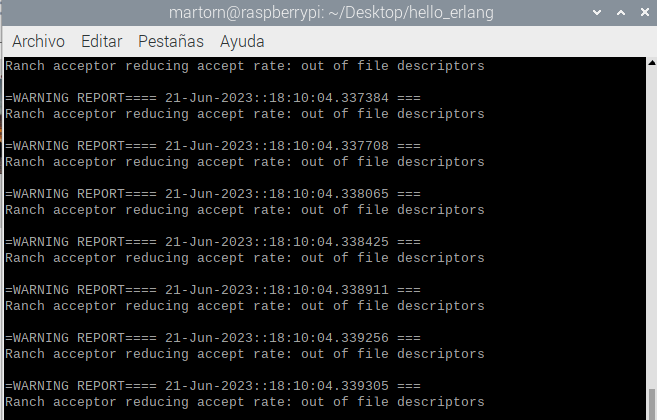
\includegraphics{images/warningServerDescriptors.png}
\caption[Warning del servidor por exceso de carga (15000 hilos)]{Warning obtenido en el terminal del servidor al someterlo a una carga de 15000 usuarios con un periodo de subida de 1, se observa el aviso de que no quedan descriptores de archivo.}%
\label{fig:warning}
\end{figure}


\begin{figure}[h]
\centering
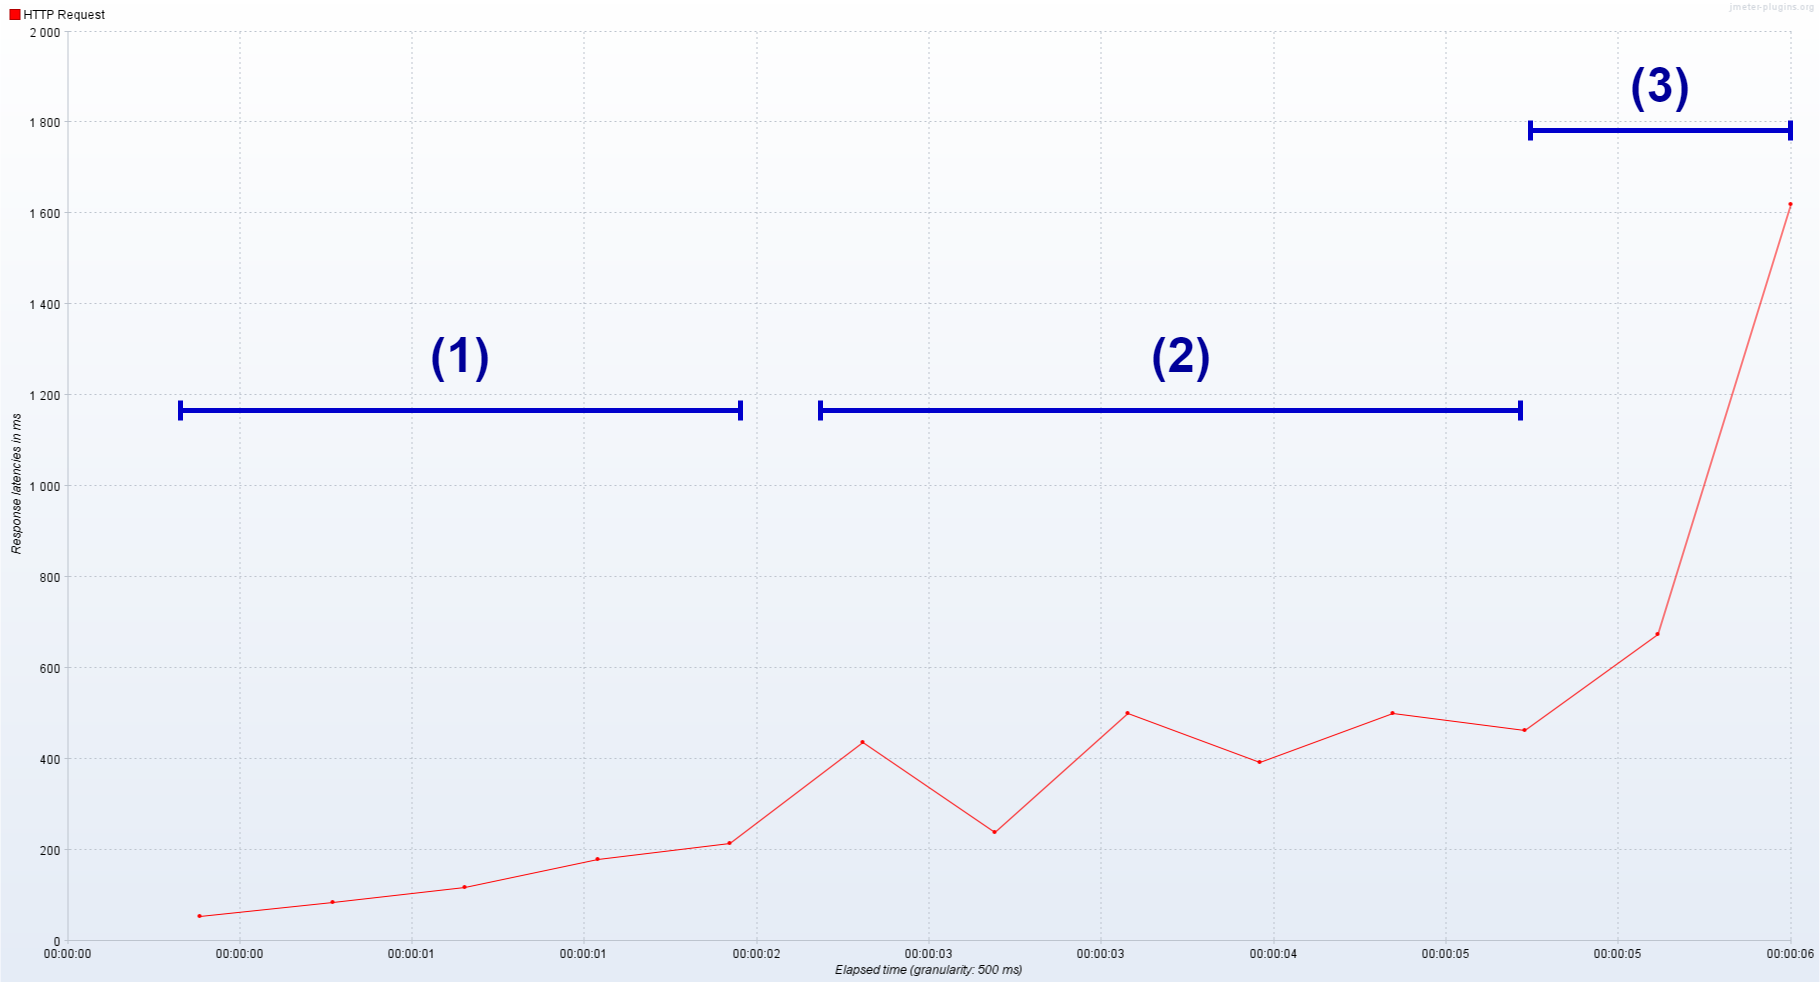
\includegraphics[scale=0.28]{images/latencia15k.png}
\caption[Evolución de la latencia con 15000 usuarios]{Evolución de la latencia en resolución de las peticiones desde 0 hasta 15000 usuarios. Eje X medido en {\ttfamily hh:mm:ss} y eje Y medido en milisegundos. La zona (1) delimita desde 0 hasta el segundo 2, zona (2) desde el 2 al segundo 5 y zona (3) del segundo 5 al final de la prueba.}%
\label{fig:latencia15k}
\end{figure}


La Tabla~\ref{tab:1500010sUser} muestra los datos más interesantes del listener \textit{Agregate Report} obtenidos con la prueba que ha lanzado peticiones de 15000 usuarios con un periodo de subida de 10 segundos. Se trata de los tiempos de respuesta medidos en milisegundos por parte de la herramienta.

A través de estos resultamos observamos que se ha obtenido un error del 0,00\% por lo que, a pesar de ser tal cantidad de usuarios (15000), al no acceder de manera simultánea sino a lo largo de 10 segundos, el servidor ha sido capaz de ir resolviendo las peticiones de manera constante sin saturarse obteniendo así un pico máximo de latencia de 148 ms y un rendimiento medio de 998.2 peticiones resueltas por segundo.

En la Figura~\ref{fig:latencia15k10s} puede observarse como la variación de la latencia ha sido constante a lo largo del tiempo dependiendo de la carga de usuarios y la revolución de peticiones a lo largo de la zona (1), entre el segundo 6 y el 7 aparece un pico algo más elevado, esto puede deberse a que en este momento la carga de peticiones sea muy elevada, al superar los 10 segundos el servidor empieza a estabilizar su tiempo de latencia y por último, al superar los 13 segundos zona (2) comienza el descenso debido a que la mayoría de peticiones ya han sido resueltas. Para poder asegurarnos de que esta teoría es correcta, podemos utilizar la Figura~\ref{fig:hilosactivos} que nos muestra los hilos activos a lo largo de la prueba, en esta gráfica observamos como, a partir del segundo 3 que encontramos el punto más elevado de hilos activos, con más de 180, estos comienzan a descender de manera escalonada hasta que, a partir del segundo 10 comienzan una bajada mucho más progresiva que se mantiene cerca de los 20 hilos activos hasta la finalización de la prueba. Estos datos indican que el servidor es capaz de resolver gran cantidad de peticiones siempre que no se supere el umbral de descriptores, de tal manera que, si la entrada de usuarios es paulatina y no simultánea, se obtienen unos rendimientos y una tasa de resolución de peticiones francamente buena. 




\begin{table}[h]
\begin{center}
\begin{tabular}{|c|c|c|c|c|c|c|c|}
\rowcolor{gray!20}
\hline
Muestras & Media & Mínimo & Máximo & \% Error & Rendimiento & KB/s Recibidos & KB/s enviados \\
\hline
15000 & 12 & 4 & 148 & 0.00\% & 998.2/s & 353.86 & 118.93 \\
\hline
\end{tabular}
\caption[Datos de <<Agregate Report>> con 15000 usuarios y 10 segundos de suboda]{Datos obtenidos por el listener <<Agregate Report>> tras las pruebas realizadas con 15000 usuarios y un tiempo de subida de 10 segundos, tiempos de respuesta en milisegundos}%
\label{tab:1500010sUser}
\end{center}
\end{table}

\begin{figure}[h]
\centering
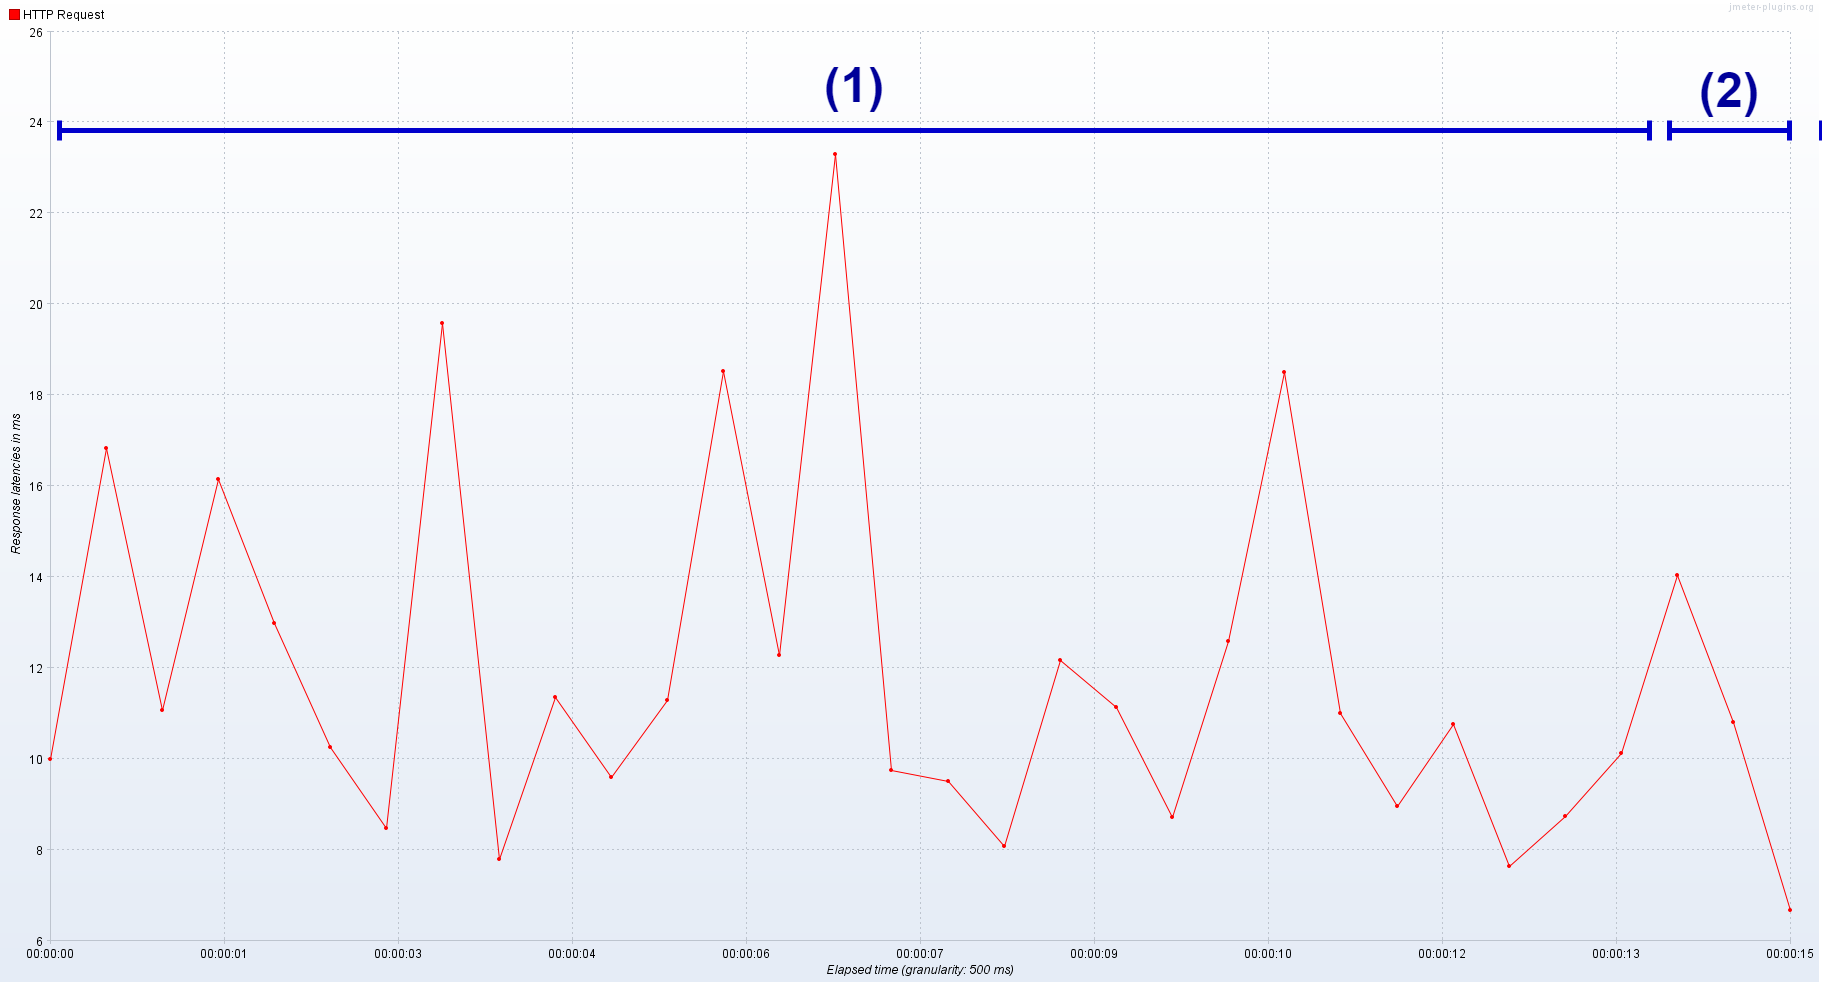
\includegraphics[scale=0.28]{images/latencia15k10s.png}
\caption[Evolución de la latencia con 15000 usuarios y 10 segundos de subida]{Evolución de la latencia en resolución de las peticiones desde 0 hasta 15000 usuarios con 10 segundos de periodo de subida. Eje X medido en {\ttfamily hh:mm:ss} y eje Y medido en milisegundos . La zona (1) delimita desde 0 hasta el segundo 14 y zona (2) desde el segundo 14 al final de la prueba.}%
\label{fig:latencia15k10s}
\end{figure}

\begin{figure}[h]
\centering
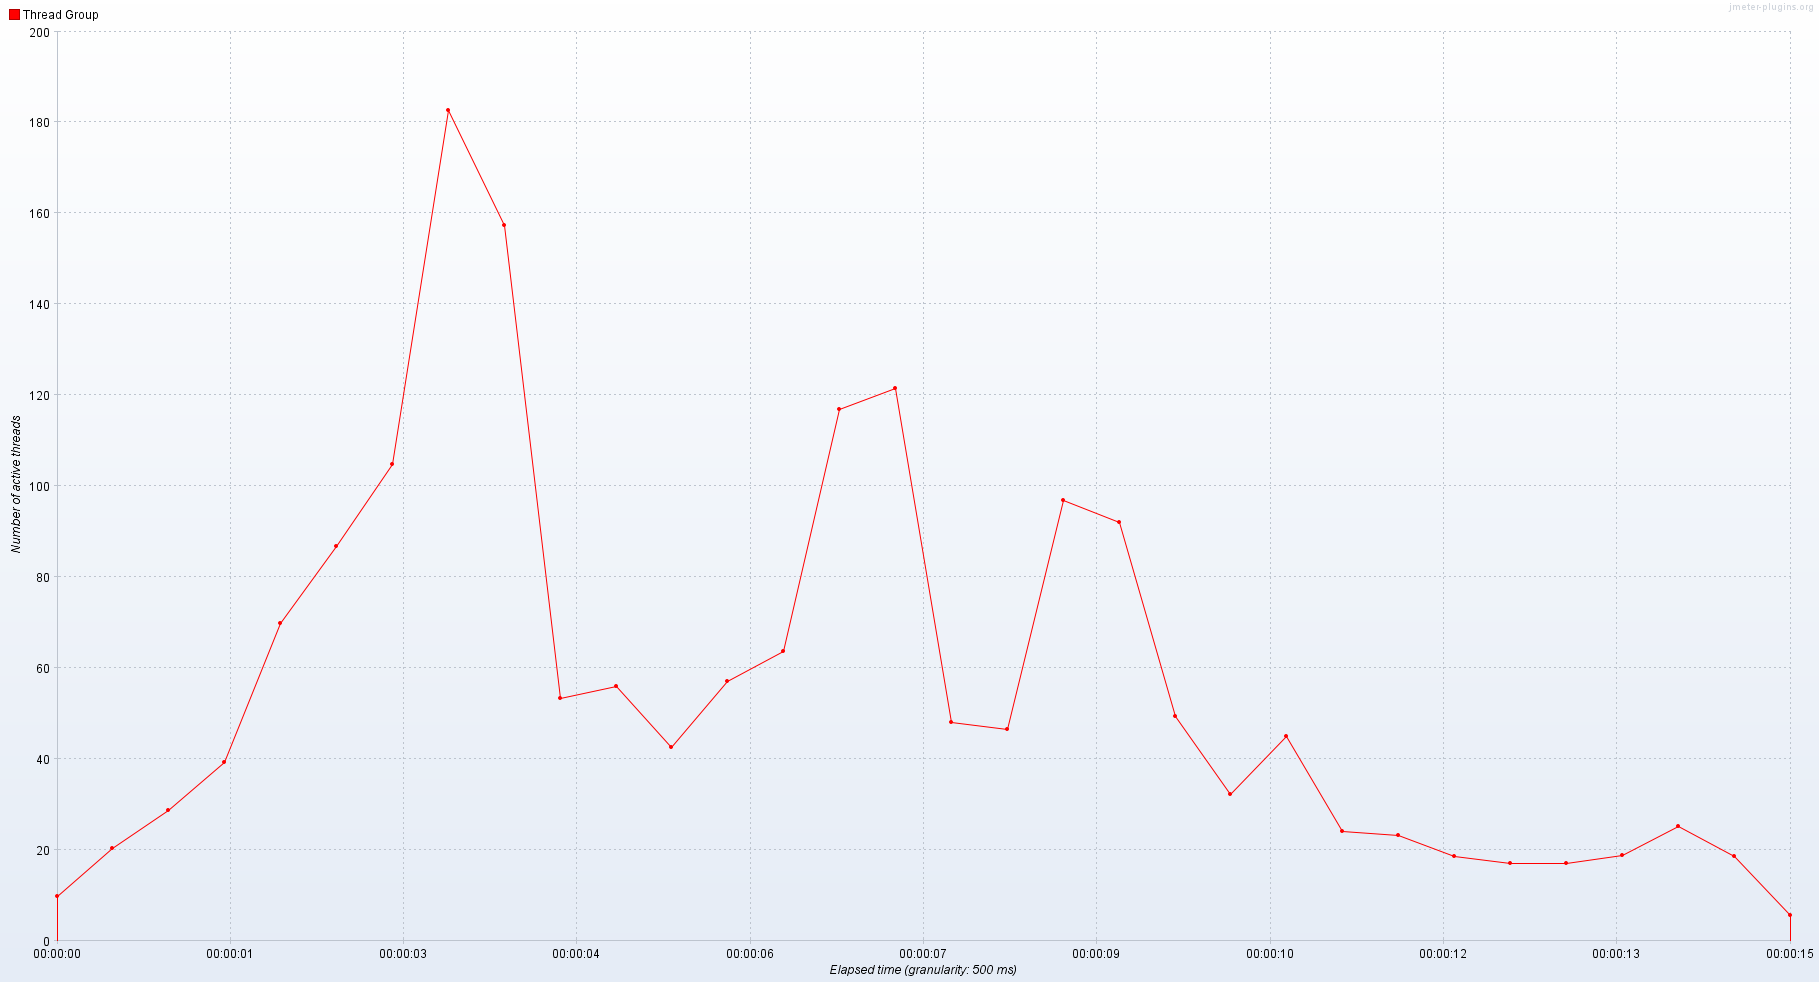
\includegraphics[scale=0.28]{images/hilosActivosGraf15k10subida.png}
\caption[Evolución de hilos activos con 15000 usuarios y 10 segundos de subida]{Evolución de los hilos activos en resolución de las peticiones desde 0 hasta 15000 usuarios con 10 segundos de periodo de subida. Eje X medido en {\ttfamily hh:mm:ss} y eje Y medido en número de hilos.}%
\label{fig:hilosactivos}
\end{figure}